\begin{frame}
\frametitle{About This Work...}

\emph{A Foundation for Efficient Indoor Distance-Aware Query Processing}.~\cite{DBLP:conf/icde/LuCJ12} \\
H.~Lu, X.~Cao, and C.~S. Jensen.\\~\\

\begin{itemize}
  \item Published at \emph{ICDE' 2012}.
  \item First time to propose a distance-aware indoor space model that integrates indoor distance seamlessly.
  \item Accompanying, efficient algorithms for computing indoor distances.
  \item Indexing framework that accommodates indoor distances.
\end{itemize}

\end{frame}

%------------------------------------------------

\begin{frame}
\frametitle{Motivation}

\begin{itemize}
  \item A variety of LBS services are useful in indoor space.
    \begin{fitemize}
      \item a museum guidance service in a complex exhibition
      \item boarding reminder service in an airport, to remind the passengers especially those far away from their gates or departures
    \end{fitemize}

  \item Such indoor LBSs will benefit from the availability of accurate indoor distances.
    \begin{fitemize}
      \item indoor space entities enable as well as constrain indoor movement, thus makes traditional space model for Euclidean/spatial network spaces unsuitable.
      \item existing indoor space models~\cite{becker2005location, li2008lattice, becker2009multilayered} pay little attention to indoor distances.
    \end{fitemize}

\end{itemize}

\end{frame}

%------------------------------------------------

\begin{frame}
\frametitle{Indoor Topology Mapping Structures}

Mapping $D2P$ maps a door $d_k$ to one or two partition pairs~\footnote{\ssize{the basic assumption that a door corresponds to two doors can be extended by converting a door to multiple doors.}} $(v_i, v_j)$ such that one can move from partition~\footnote{\ssize{a partition indicates a room, a hallway or a staircase.}} $v_i$ to partition $v_j$ through door $d_k$:
\pause
\begin{equation}
 D2P: \mathcal{S}_{door} \rightarrow 2^{\mathcal{S}_{partition}} \times 2^{\mathcal{S}_{partition}}
\end{equation}
\pause
For \emph{enterable partition} of door $d_k$:
\pause
\begin{equation}
 D2P_{\sqsupset}: \mathcal{S}_{door} \rightarrow 2^{\mathcal{S}_{partition}}
\end{equation}
\pause
For \emph{leaveable partition} of door $d_k$:
\pause
\begin{equation}
 D2P_{\sqsubset}: \mathcal{S}_{door} \rightarrow 2^{\mathcal{S}_{partition}}
\end{equation}
\end{frame}

%------------------------------------------------

\begin{frame}
\frametitle{Indoor Topology Mapping Structures}


The mapping $P2D_{\sqsupset}$ maps a partition $v$ to all the doors through which one can enter $v$:
\pause
\begin{equation}
 P2D_{\sqsupset}: \mathcal{S}_{partition} \rightarrow 2^{\mathcal{S}_{door}}
\end{equation}
\pause
The mapping $P2D_{\sqsubset}$ maps a partition $v$ to all the doors through which one can leave $v$:
\pause
\begin{equation}
 P2D_{\sqsubset}: \mathcal{S}_{partition} \rightarrow 2^{\mathcal{S}_{door}}
\end{equation}
\pause
The mapping $P2D$ is used when there's no need to differentiate the directionality:
\pause
\begin{equation}
 P2D(v_i): P2D_{\sqsupset}(v_i) \cup P2D_{\sqsubset}(v_i)
\end{equation}
\end{frame}

%------------------------------------------------

\begin{frame}
\frametitle{Accessibility Base Graph}

\begin{columns}[c]

  \column{0.52\textwidth}
  \vspace{-15pt}
  \begin{figure}[tb]
    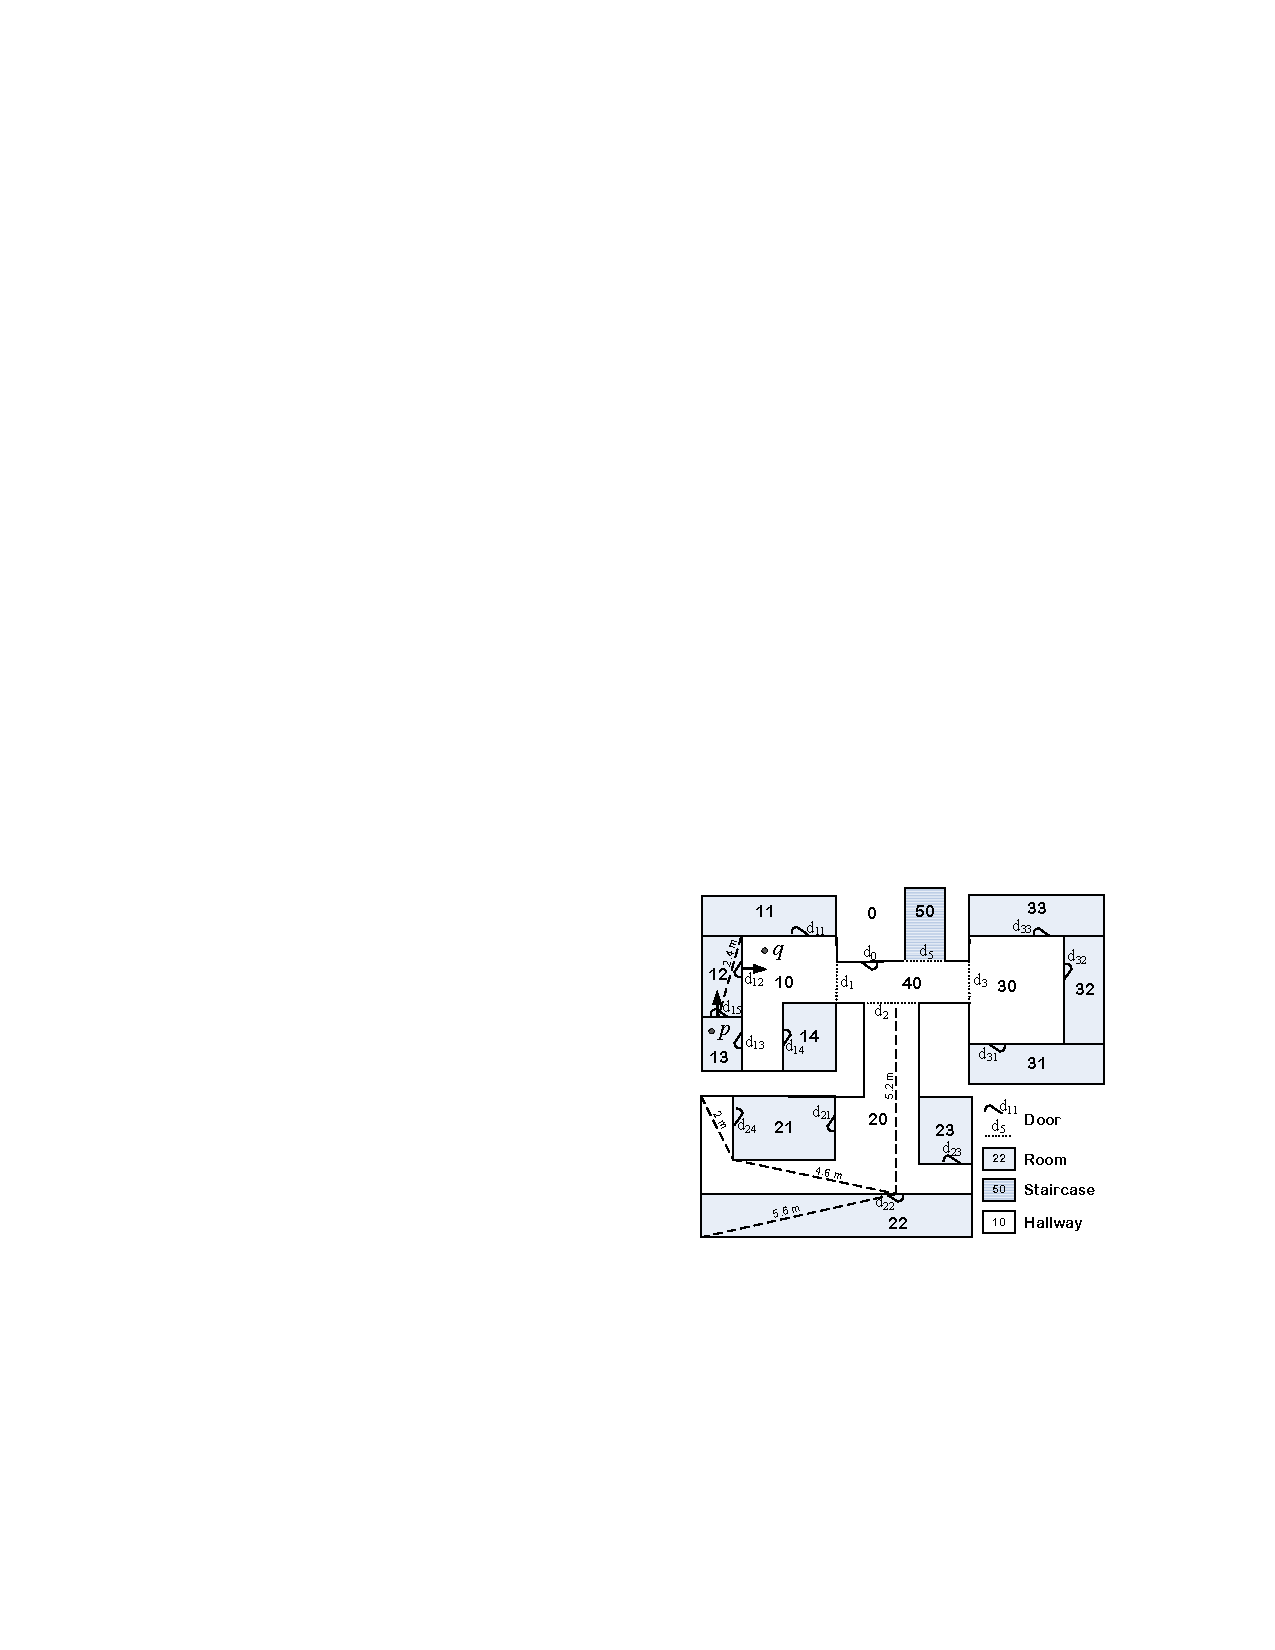
\includegraphics[width=0.85\columnwidth]{figures/2-5/2-5-1.pdf}
  \end{figure}
  \begin{example}
    \textrm{
    \ssize{
      $D2P_{\sqsupset}(d_{12}) = \{ v_{10}\}$, $D2P_{\sqsubset}(d_{12}) = \{ v_{12}\}$
      $P2D_{\sqsupset}(v_{13}) = \{ d_{13}\}$, $P2D_{\sqsubset}(v_{13}) = \{ d_{13}, d_{15}\}$
    }
    }
  \end{example}

  \column{0.48\textwidth}
  \vspace{-15pt}
  \begin{figure}[tb]
    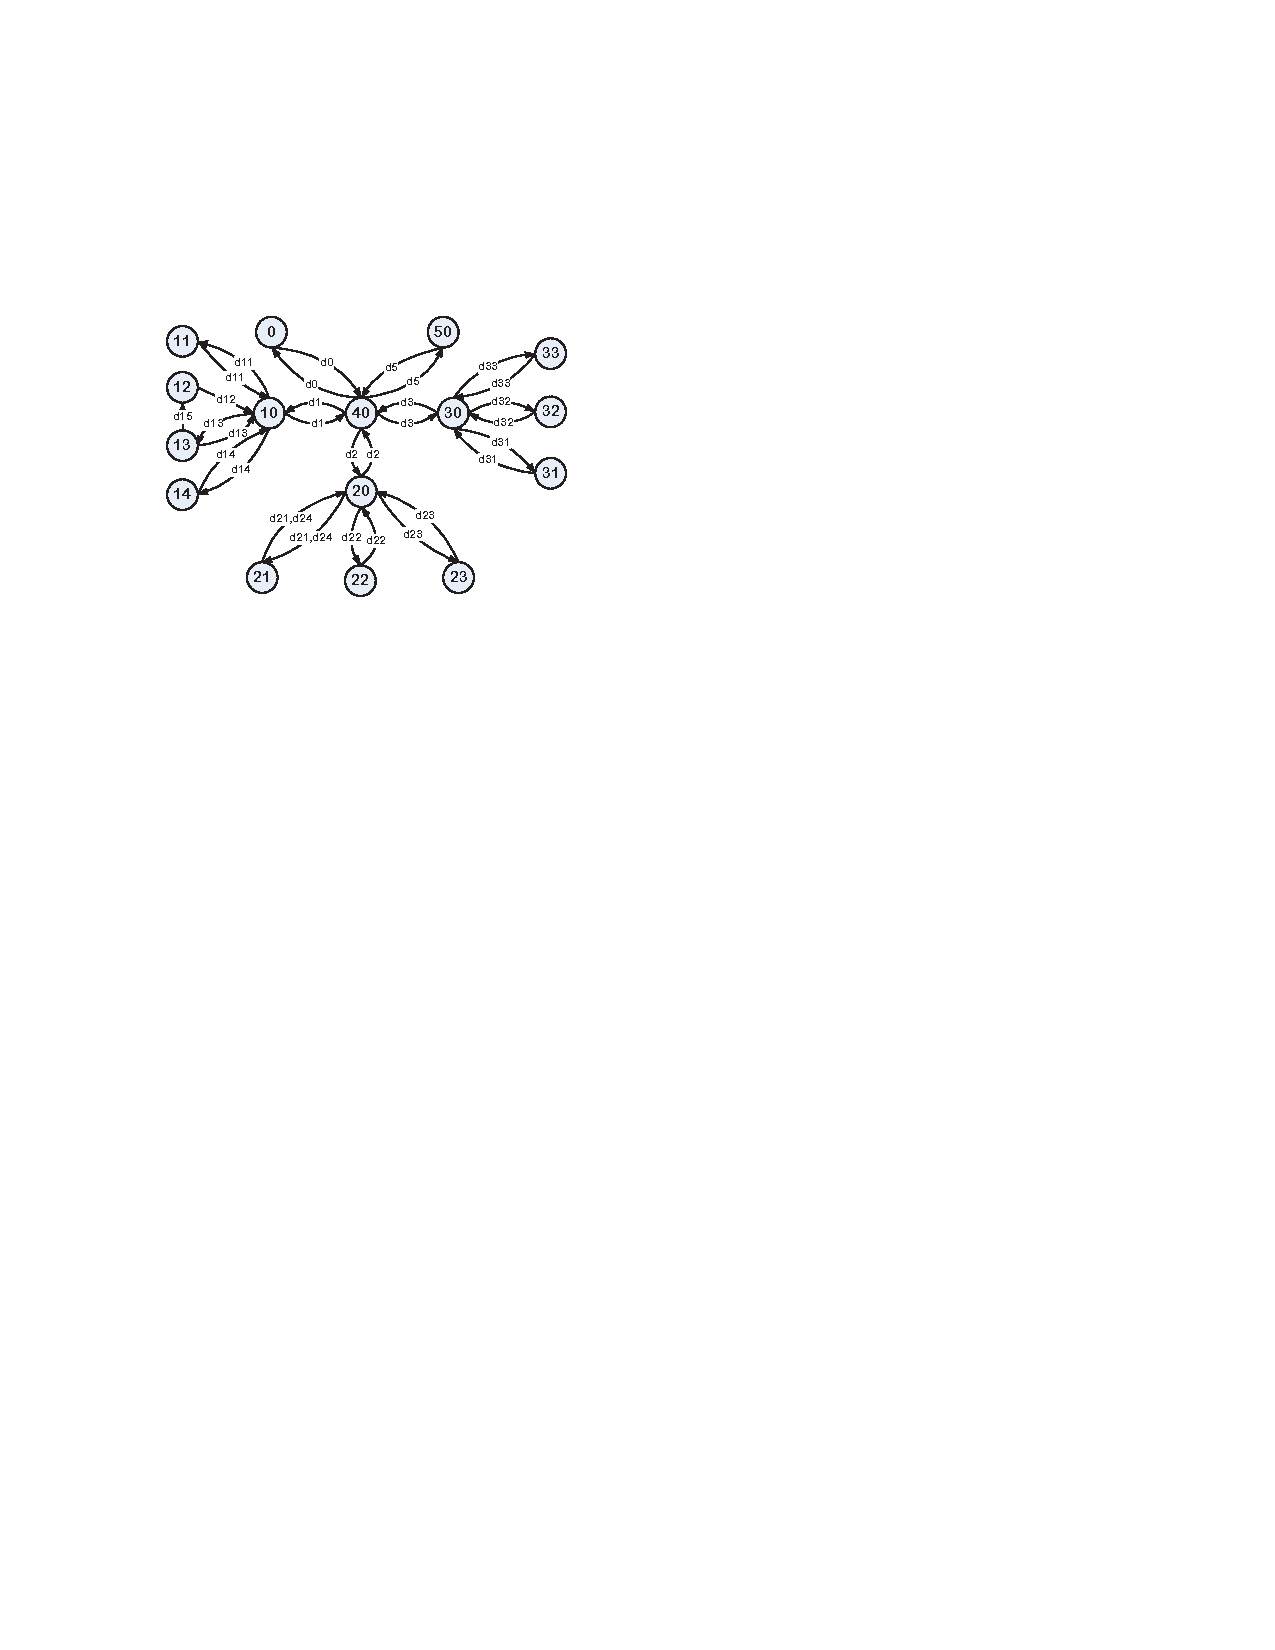
\includegraphics[width=0.8\columnwidth]{figures/2-5/2-5-2.pdf}
  \end{figure}
  \vspace{-10pt}
  \begin{block}{Accessibility Base Graph}
    \textrm{
    \ssize{
    \begin{itemize}
      \item $G_{accs} = \{V, E_a, L\}$
      \item $V = \mathcal{S}_{partition}$ is the set of vertices
      \item $E_a = \{ (v_i, v_j, d_k) | (v_i, v_j) \in D2P(d_k) \}$ is the set of labeled, directed edges
      \item $L = \mathcal{S}_{door}$ is the set of edge labels
    \end{itemize}
    }
    }
  \end{block}

\end{columns}

\end{frame}

%------------------------------------------------

\begin{frame}
\frametitle{Distance-Aware Model}

\fsize{\textrm{The $G_{accs}$ graph does not capture indoor distance information. \conceptbf{Extended Graph Model} is proposed to integrate indoor distances into the graph in a seamless way. \emph{Minimum Indoor Walking Distance}(MIWD) is used. }}

\begin{block}{Extended Graph Model $G_{dist} = \{ V, E_a, L, f_{dv}, f_{d2d} \}$}
  \textrm{
  \begin{sitemize}
    \item $V = \mathcal{S}_{partition}$ is the set of vertices
    \item $E_a = G_{accs}.E_a$
    \item $L = \mathcal{S}_{door}$ is the set of edge labels
    \item $f_{dv} = \mathcal{S} \times V \rightarrow \mathcal{R} \cup \{ \infty \}$ maps an edge to a distance value.
    \begin{equation*}
      f_{dv} = \left\{\begin{matrix}
                \max_{p \in v_j}|| d_i, p || , & if~~ v_j \in D2P_{\sqsupset};
                \\
                \infty , & otherwise.
                \end{matrix}\right.
    \end{equation*}
    \item $f_{d2d} = V \times \mathcal{S}_{door} \times \mathcal{S}_{door} \rightarrow \mathcal{R} \cup \{ \infty \}$ maps a 3-tuple to a distance value.
    \begin{equation*}
      f_{dv} = \left\{\begin{matrix}
                || d_i, d_j ||_{v_k} , & if~~ d_i \in P2D_{\sqsupset}(v_k) and d_j \in P2D_{\sqsubset}(v_k);
                \\
                \infty , & if~~ d_i = d_j and d_i,d_j \in P2D(v_k);
                \\
                0 , & otherwise.
                \end{matrix}\right.
    \end{equation*}
  \end{sitemize}
  }
\end{block}

\end{frame}

%------------------------------------------------

\begin{frame}
\frametitle{Computation: \emph{door-to-door distance}}

\begin{columns}[c]

  \column{0.52\textwidth}
  \begin{figure}[tb]
    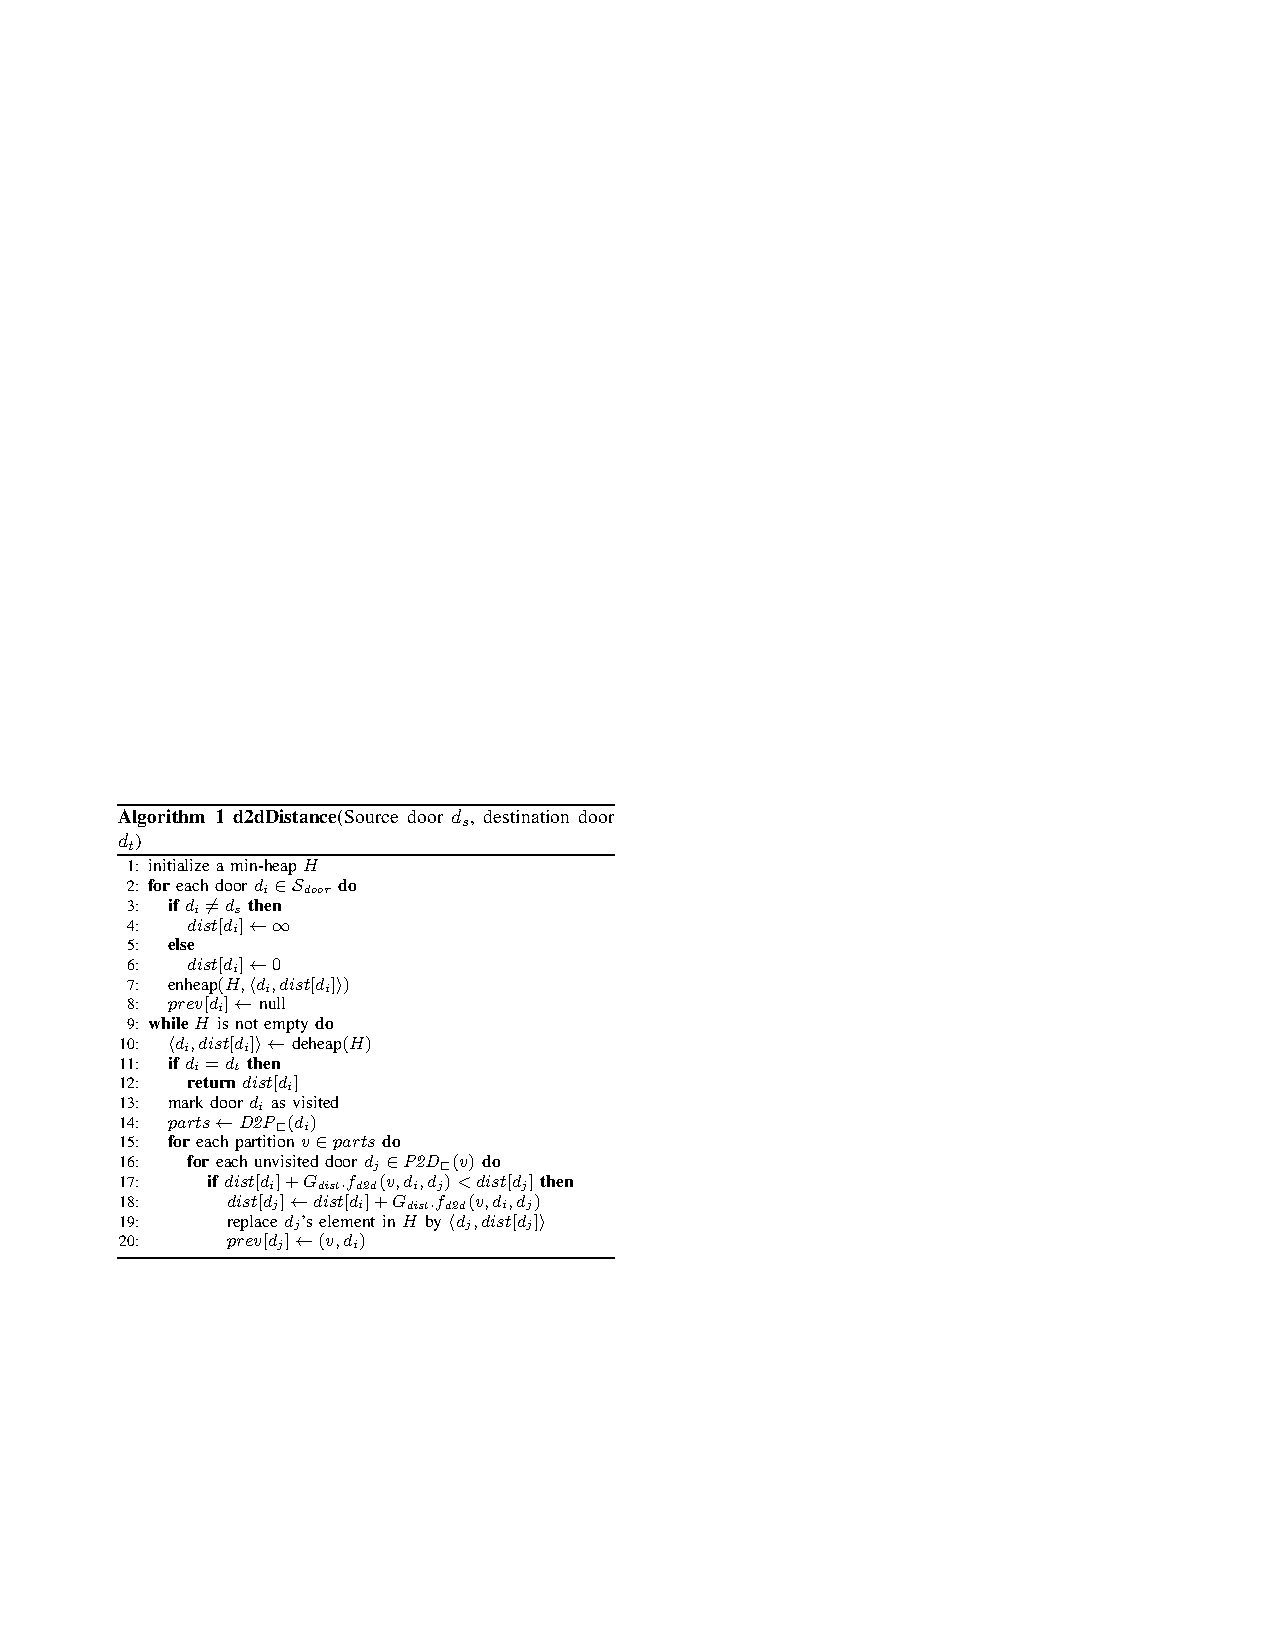
\includegraphics[width=\columnwidth]{figures/2-5/2-5-3.pdf}
  \end{figure}

  \column{0.48\textwidth}
  \ssize{
  \begin{enumerate}
    \item $d_t$ as source door, $d_s$ as destination door, $d2dDistance(d_t, d_s)$ finds the minimum walking distance in a \emph{Dijkstra} way.
    \item $dist[d_j]$ stores the current shorest path distance from souce $d_s$ to a door $d_j$.
    \item $prev[d_j]$ stores the corresponding previous partition and door pair $(v,d_i)$ through which the algorithm visits the current door $d_j$.
  \end{enumerate}
  }

\end{columns}

\end{frame}

%------------------------------------------------

\begin{frame}
\frametitle{Computation: \emph{point-to-point distance} (I)}

\begin{columns}[c]

  \column{0.5\textwidth}
  \begin{figure}[tb]
    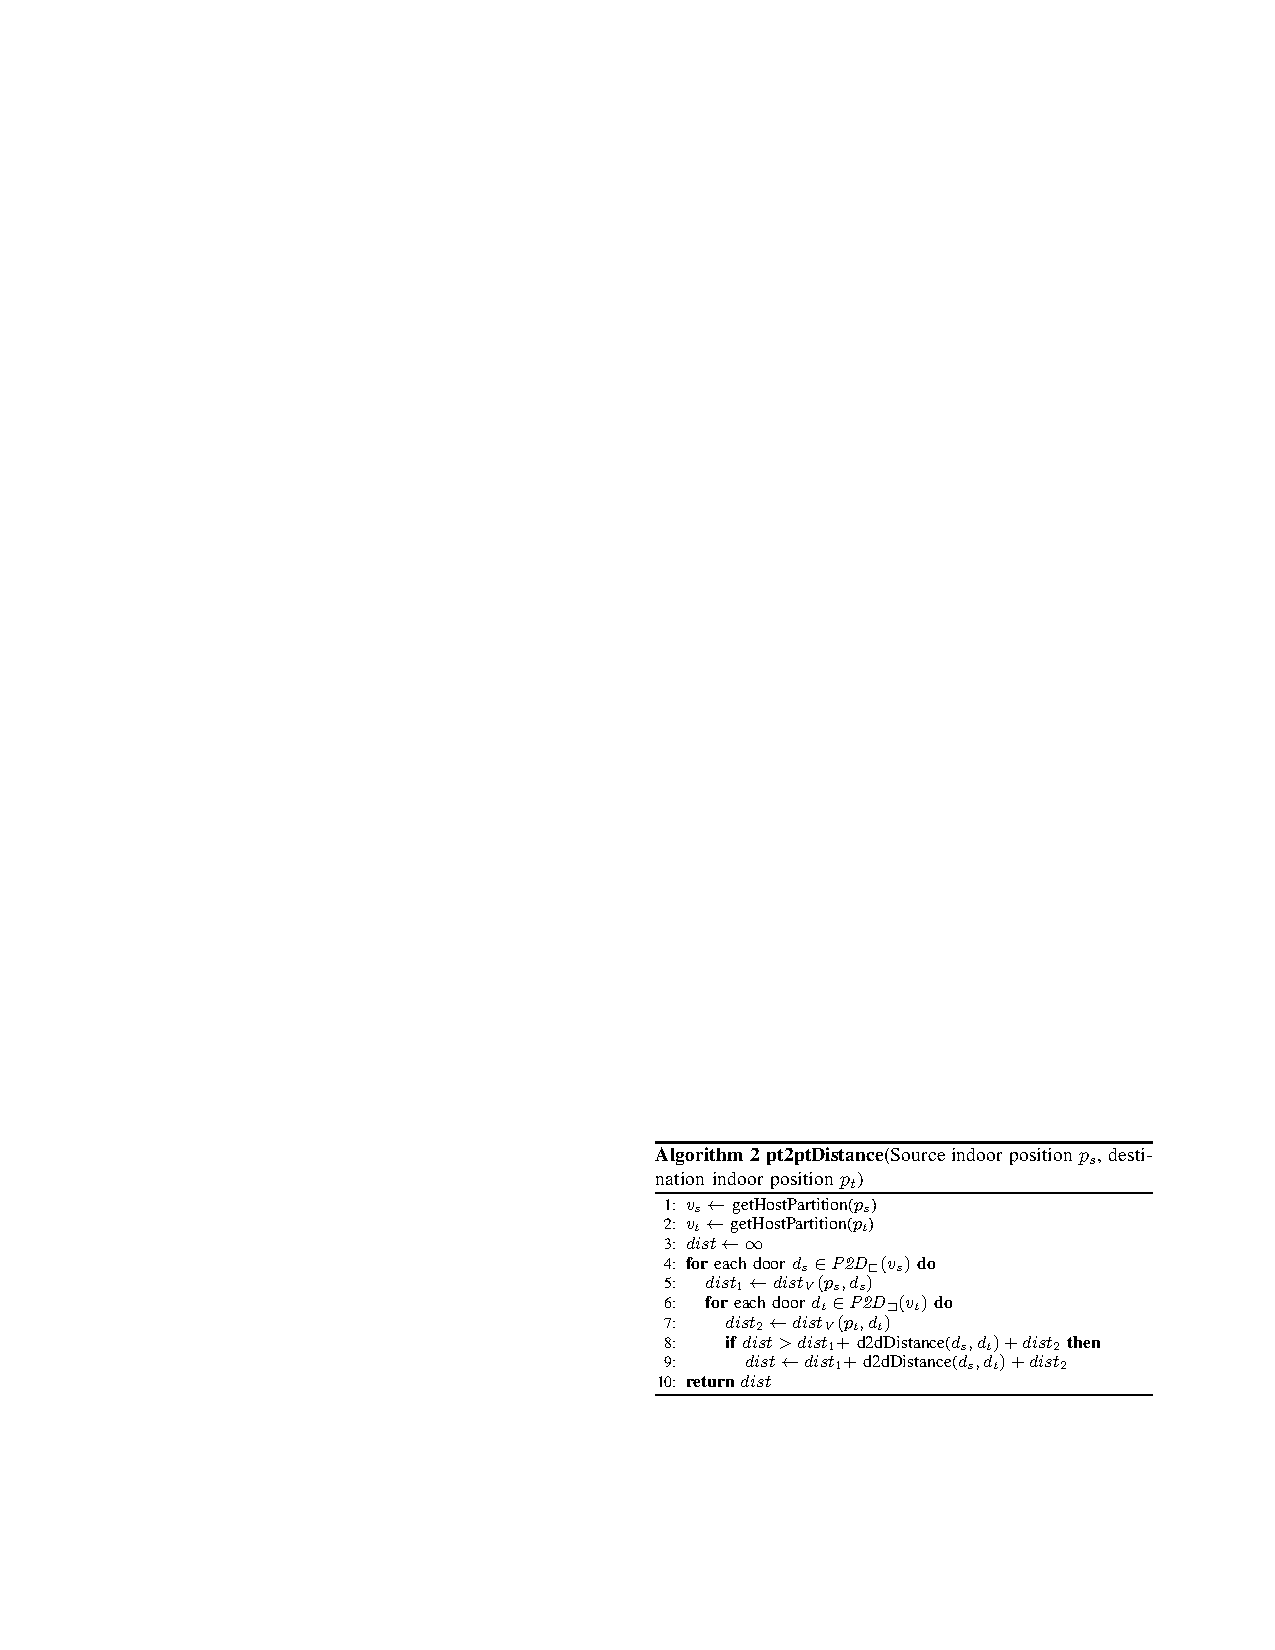
\includegraphics[width=\columnwidth]{figures/2-5/2-5-4.pdf}
  \end{figure}

  \column{0.5\textwidth}
  \ssize{
  \begin{enumerate}
    \item $getHostPartition(p)$ returns the partition that contains $p$.
    \item $dist_V:P \times \mathcal{S}_{door} \rightarrow \mathcal{R} \cup \{ \infty \}$ returns the shortest intra-partition distance between a position $p$ and a door $d$, i.e., the minimum distance one must walk to get from position $p$ to door $d$ without leaving $p$'s host partition.
    \item minimum door-to-door distance from each door $d_s$ in $P2D_{\sqsubset}(d_s)$ to each door $P2D_{\sqsupset}(d_t)$ is computed.
    \item intra-partition distances $dist_V(p_s,d_s)$ and $dist_V(p_t,d_t)$ are added to that distance to get one possible position-to-position distance.
    \item the minimum is returned as the result.
  \end{enumerate}
  }

\end{columns}

\end{frame}

%------------------------------------------------

\begin{frame}
\frametitle{Computation: \emph{point-to-point distance} (II)}

\begin{columns}[c]

  \column{0.4\textwidth}
  \begin{figure}[tb]
    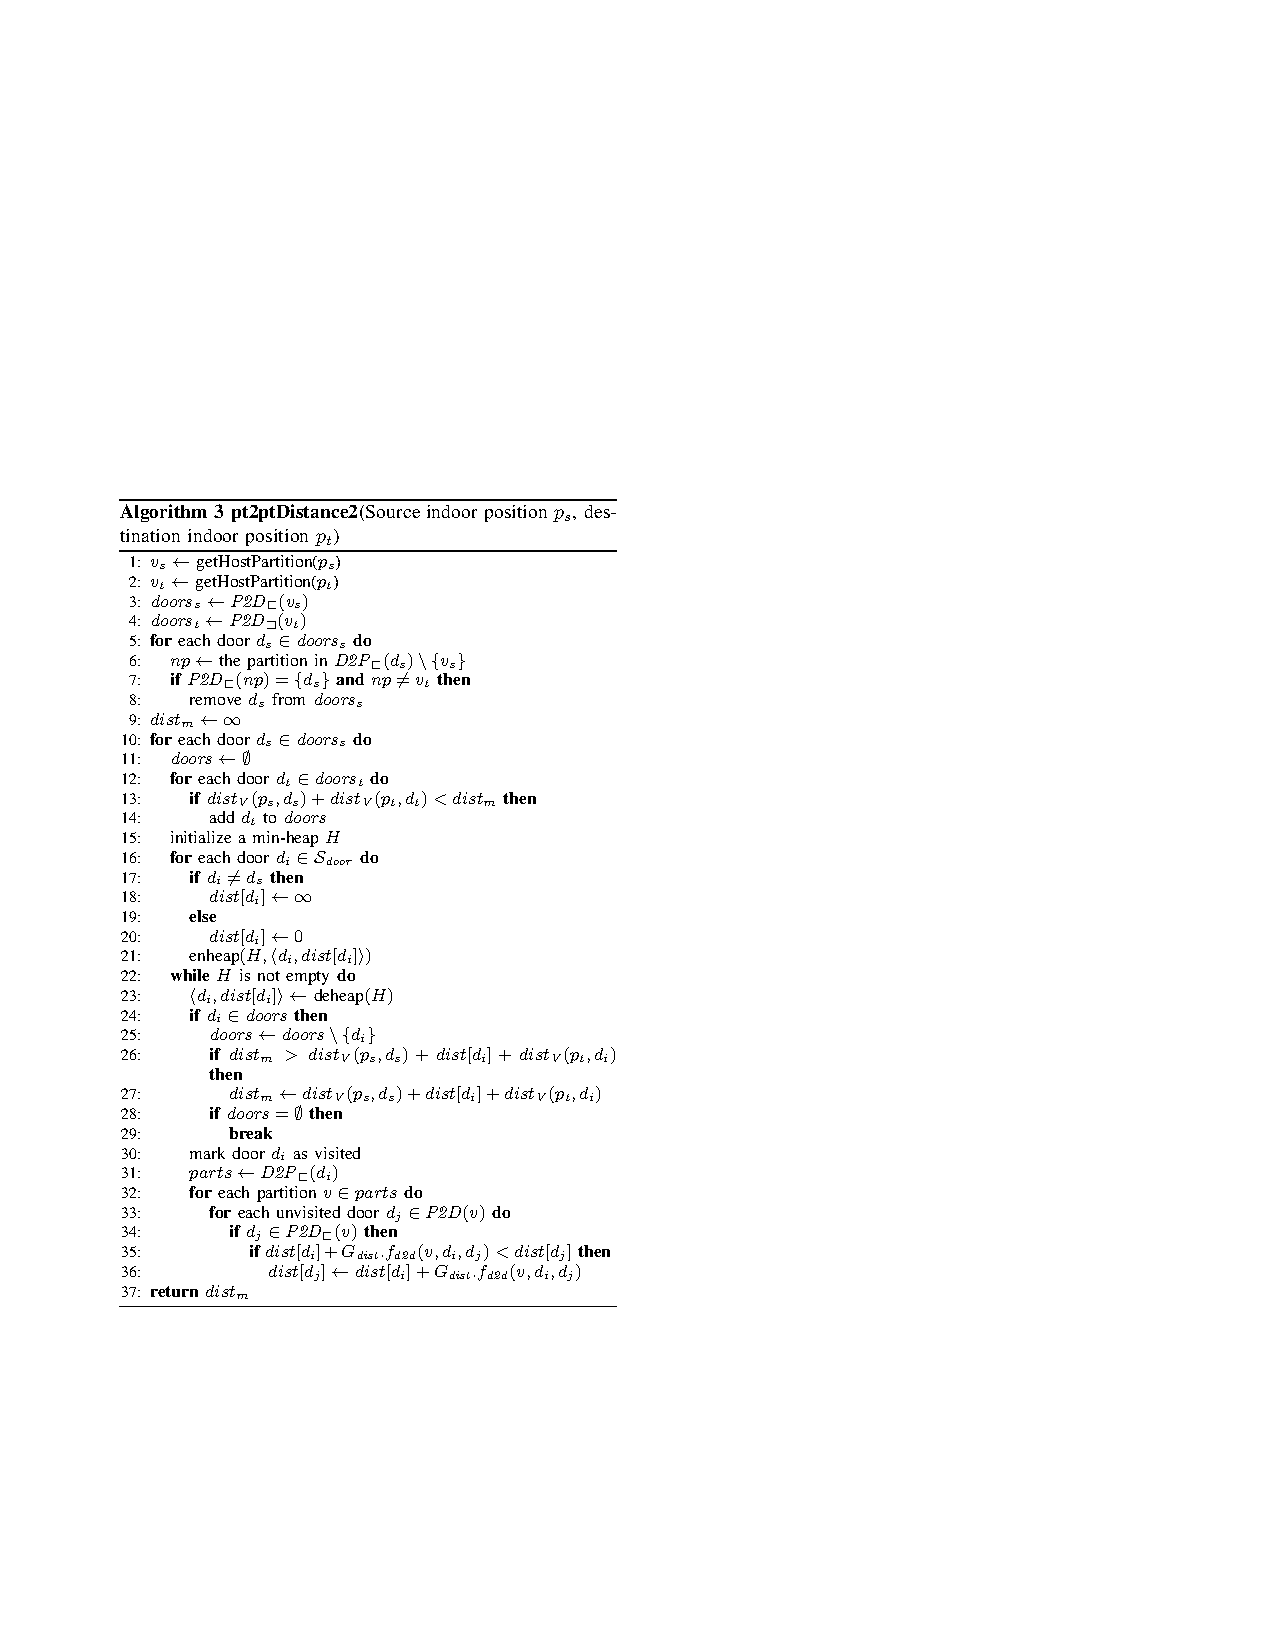
\includegraphics[width=\columnwidth]{figures/2-5/2-5-5.pdf}
  \end{figure}

  \column{0.6\textwidth}
  \ssize{
  \begin{enumerate}
    \item lines 1--4: $doors_s$($doors_t$) is initialized to contain all leaving(entering) doors of the source(destination) partition $v_s$($v_t$).
    \item lines 5--8: a door $d_s$ in $doors_s$ is excluded if it leads to a non-destination partition that has $d_s$ as its sole leaving door.
    \item lines 11--14: for each source door $d_s$, initialize a set $doors$, excluding any destination door $d_t$ that is too far away compared to current shortest distance $dist_m$.
    \item lines 15--36: follows the spirit of \emph{Dijkstra}, only visits those doors that allow objects to move out(line 34), also updates the current shortest distance $dist_m$ when a shorter one is found.
    \item the current expansion for a door $d_s$ terminates when set $doors$ becomes empty.
  \end{enumerate}
  }

\end{columns}

\end{frame}


%------------------------------------------------

\begin{frame}
\frametitle{Computation: \emph{point-to-point distance} (III)}

\begin{columns}[c]

  \column{0.52\textwidth}
  \begin{figure}[tb]
    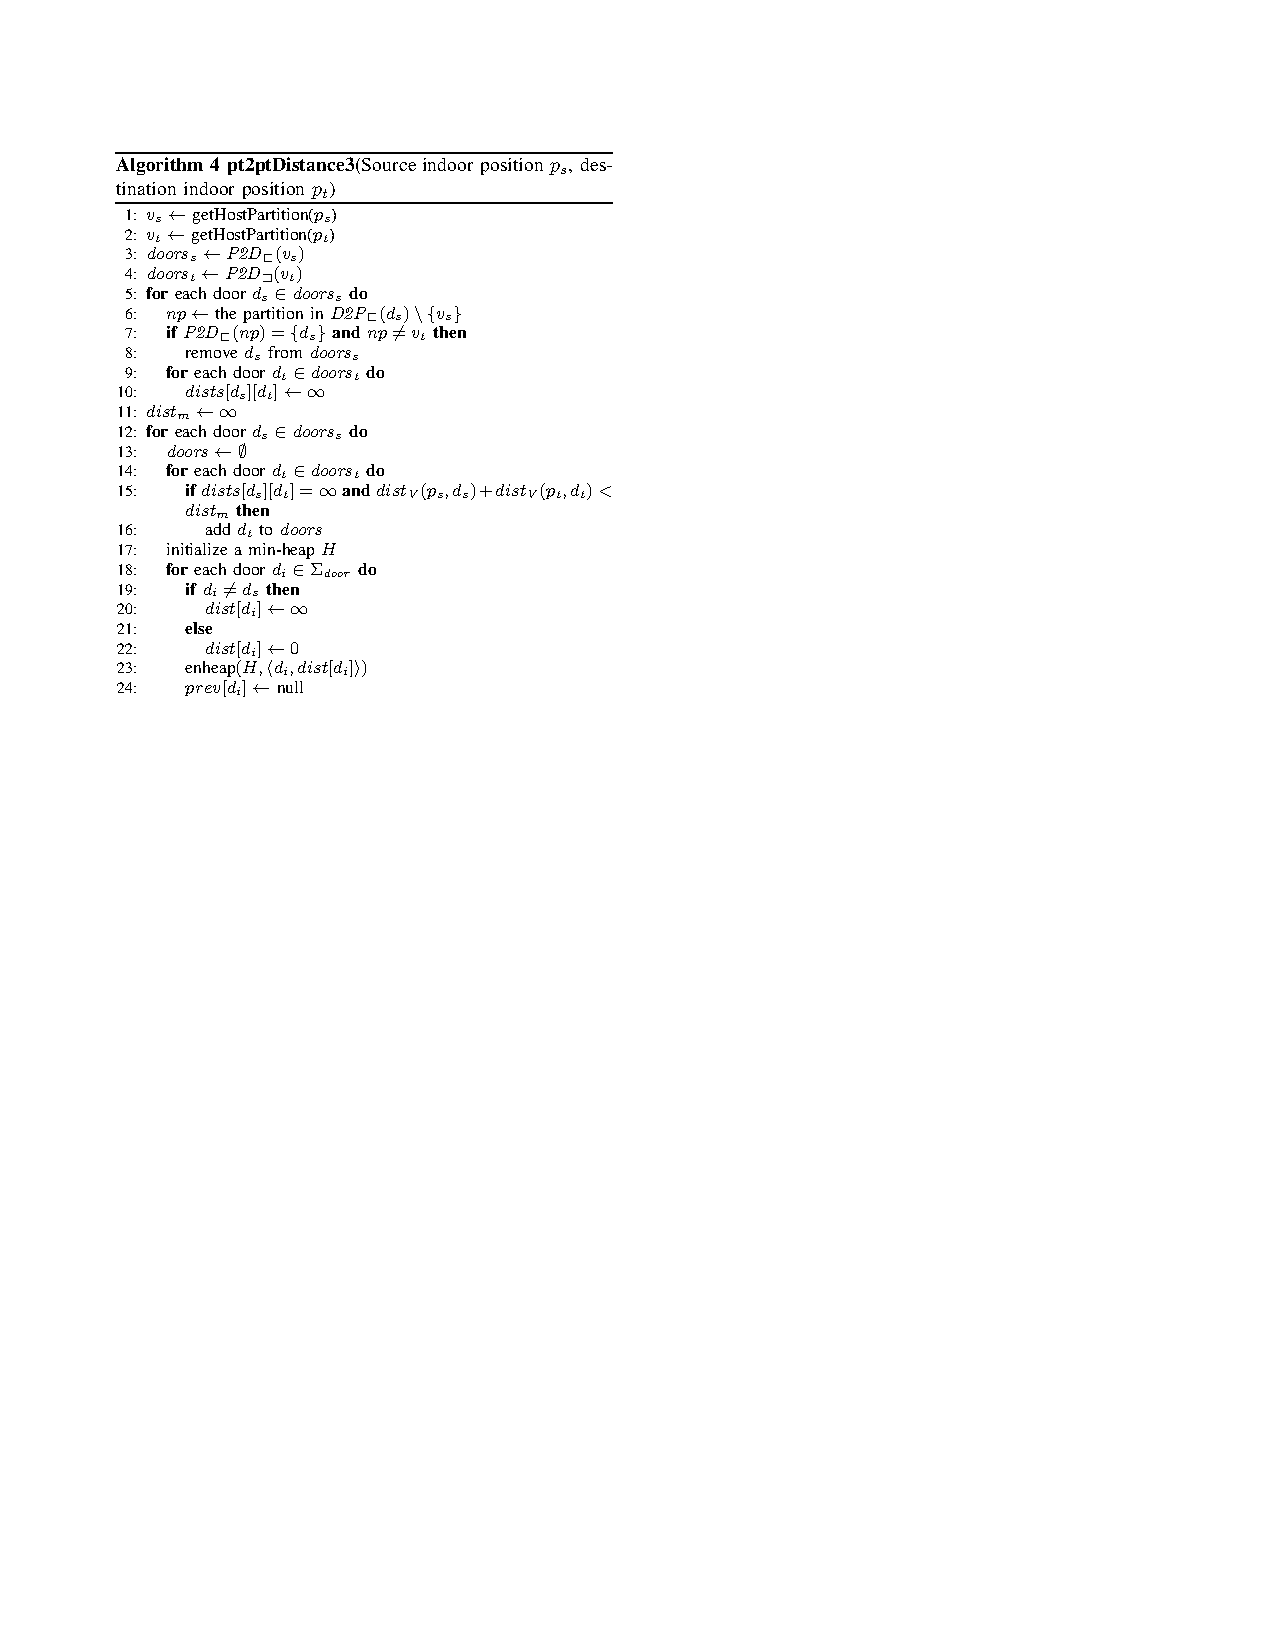
\includegraphics[width=\columnwidth]{figures/2-5/2-5-6.pdf}
  \end{figure}

  \column{0.48\textwidth}
  \ssize{
  \begin{enumerate}
    \item lines 1--8: initialize as same as the version of \emph{pt2ptDistance2}.
    \item lines 9--10: a two-dimensional array $dists[d_i][d_j]$ is employed to store the currently shortest indoor distance from source door $d_i$ to destination door $d_j$.
    \item line 15: the condition whether $dist[d_s][d_t]$ is infinity is check together with $dist_{V}(p_s,d_s) + dist_{V}(p_t,d_t) < dist_m $.
    \item line 24: initialize $prev[d_i]$ as empty.
  \end{enumerate}
  }

\end{columns}

\end{frame}

%------------------------------------------------

\begin{frame}
\frametitle{Computation: \emph{point-to-point distance} (III)}

\begin{columns}[c]

  \vspace{-25pt}
  \column{0.44\textwidth}
  \begin{figure}[tb]
    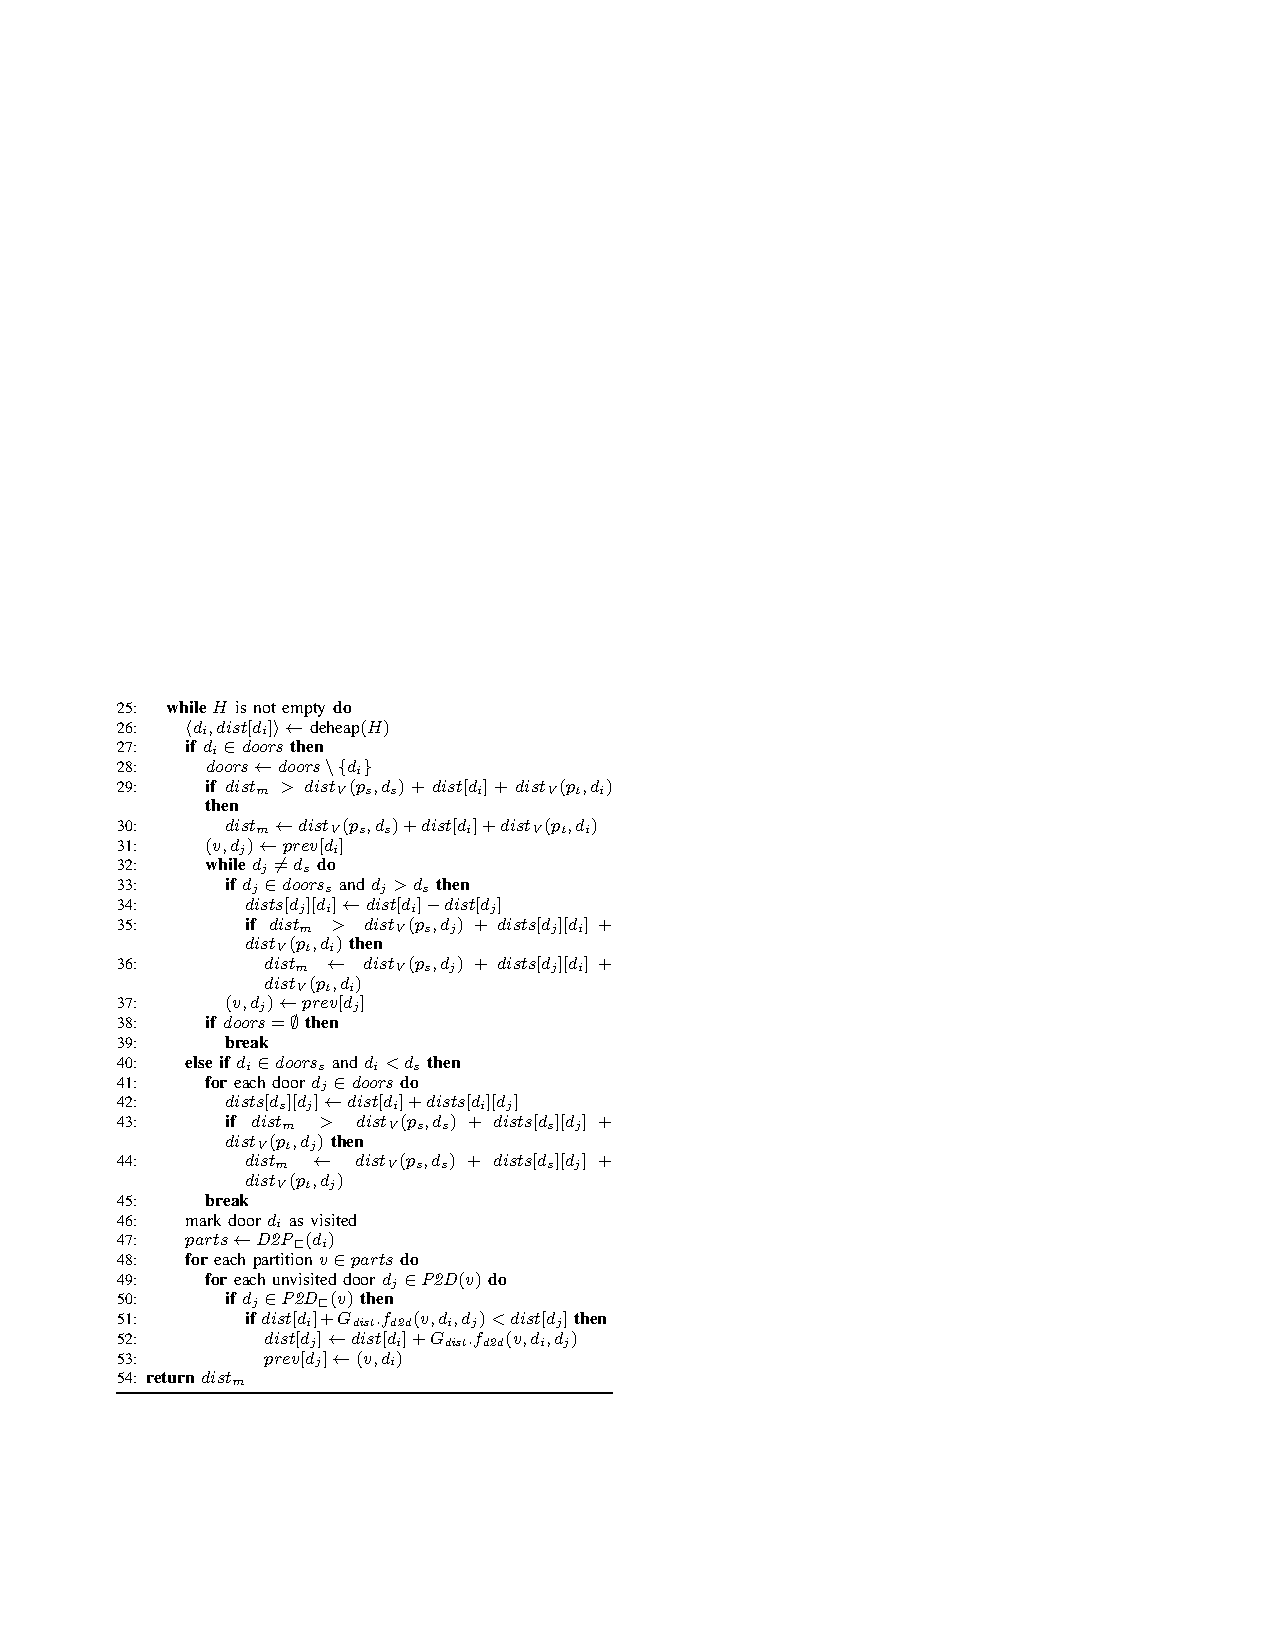
\includegraphics[width=\columnwidth]{figures/2-5/2-5-7.pdf}
  \end{figure}

  \column{0.56\textwidth}
  \ssize{
  \begin{enumerate}
    \item lines 26--31: when a destination door $door_i$ is popped from priority queue $H$ and processed, its previous door $d_j$ on the shortest path is obtained.
    \item line 32: backward optimization is continued until the current source door $d_s$ is reached.
    \item lines 33--34: if door $d_j$ is a source door and it has not been processed by the for-loop, the shortest distance from $d_j$ to destination door $d_i$ is stored in $dist[d_j][d_i]$.
    \item lines 35--36: shortest indoor distance from the source position to the destination is updated if necessary.
    \item lines 40--45: a similar optimization also applies to the forward direction. If $d_i$ popped from $H$ is a source door and processed before the current for-loop, the distance can be directly used.
  \end{enumerate}
  }

\end{columns}

\end{frame}

%------------------------------------------------

\begin{frame}
\frametitle{Indoor Distance-Aware Indexes}

\begin{definition}[Door-to-Door Distance Matrix]
\textrm{
\ssize{
an $N$-by-$N$ matrix, denoted as $M_{d2d}$, where $N = |\mathcal{S}_{doors}|$ is the total number of doors.Without loss of generality, suppose $1 \leq d_i \leq d_j \leq N$, we have:\\
1) $M_{d2d}[d_i,d_i] = 0$;\\
2) $M_{d2d}[d_i,d_j] = d2dDistance(d_i,d_j)$;\\
3) $M_{d2d}[d_i,d_j]$ may differ from $M_{d2d}[d_j,d_i]$ due to the directed doors.
}}
\end{definition}

\vspace{-10pt}
\begin{columns}[c]

  \vspace{-10pt}
  \column{0.36\textwidth}
  \begin{figure}[tb]
    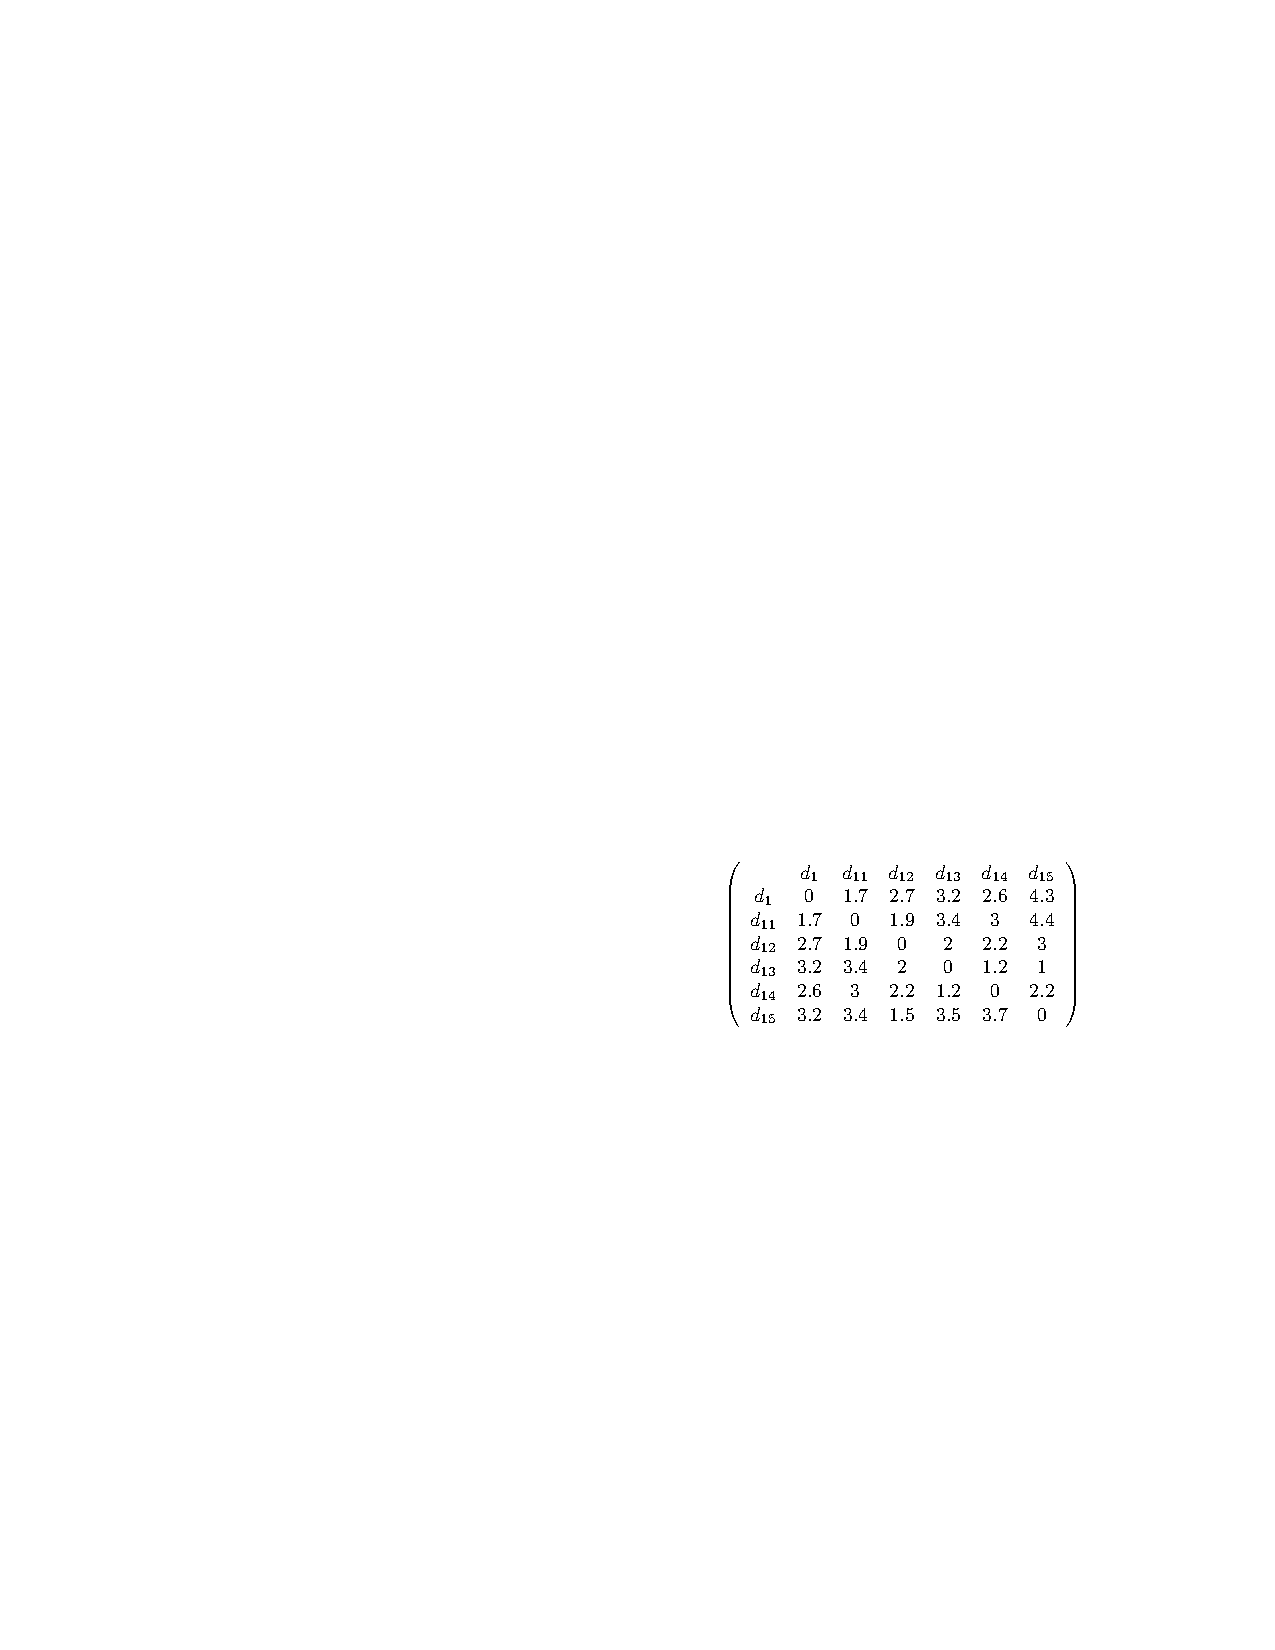
\includegraphics[width=\columnwidth]{figures/2-5/2-5-8.pdf}
  \end{figure}

  \vspace{-10pt}
  \column{0.36\textwidth}
  \begin{figure}[tb]
    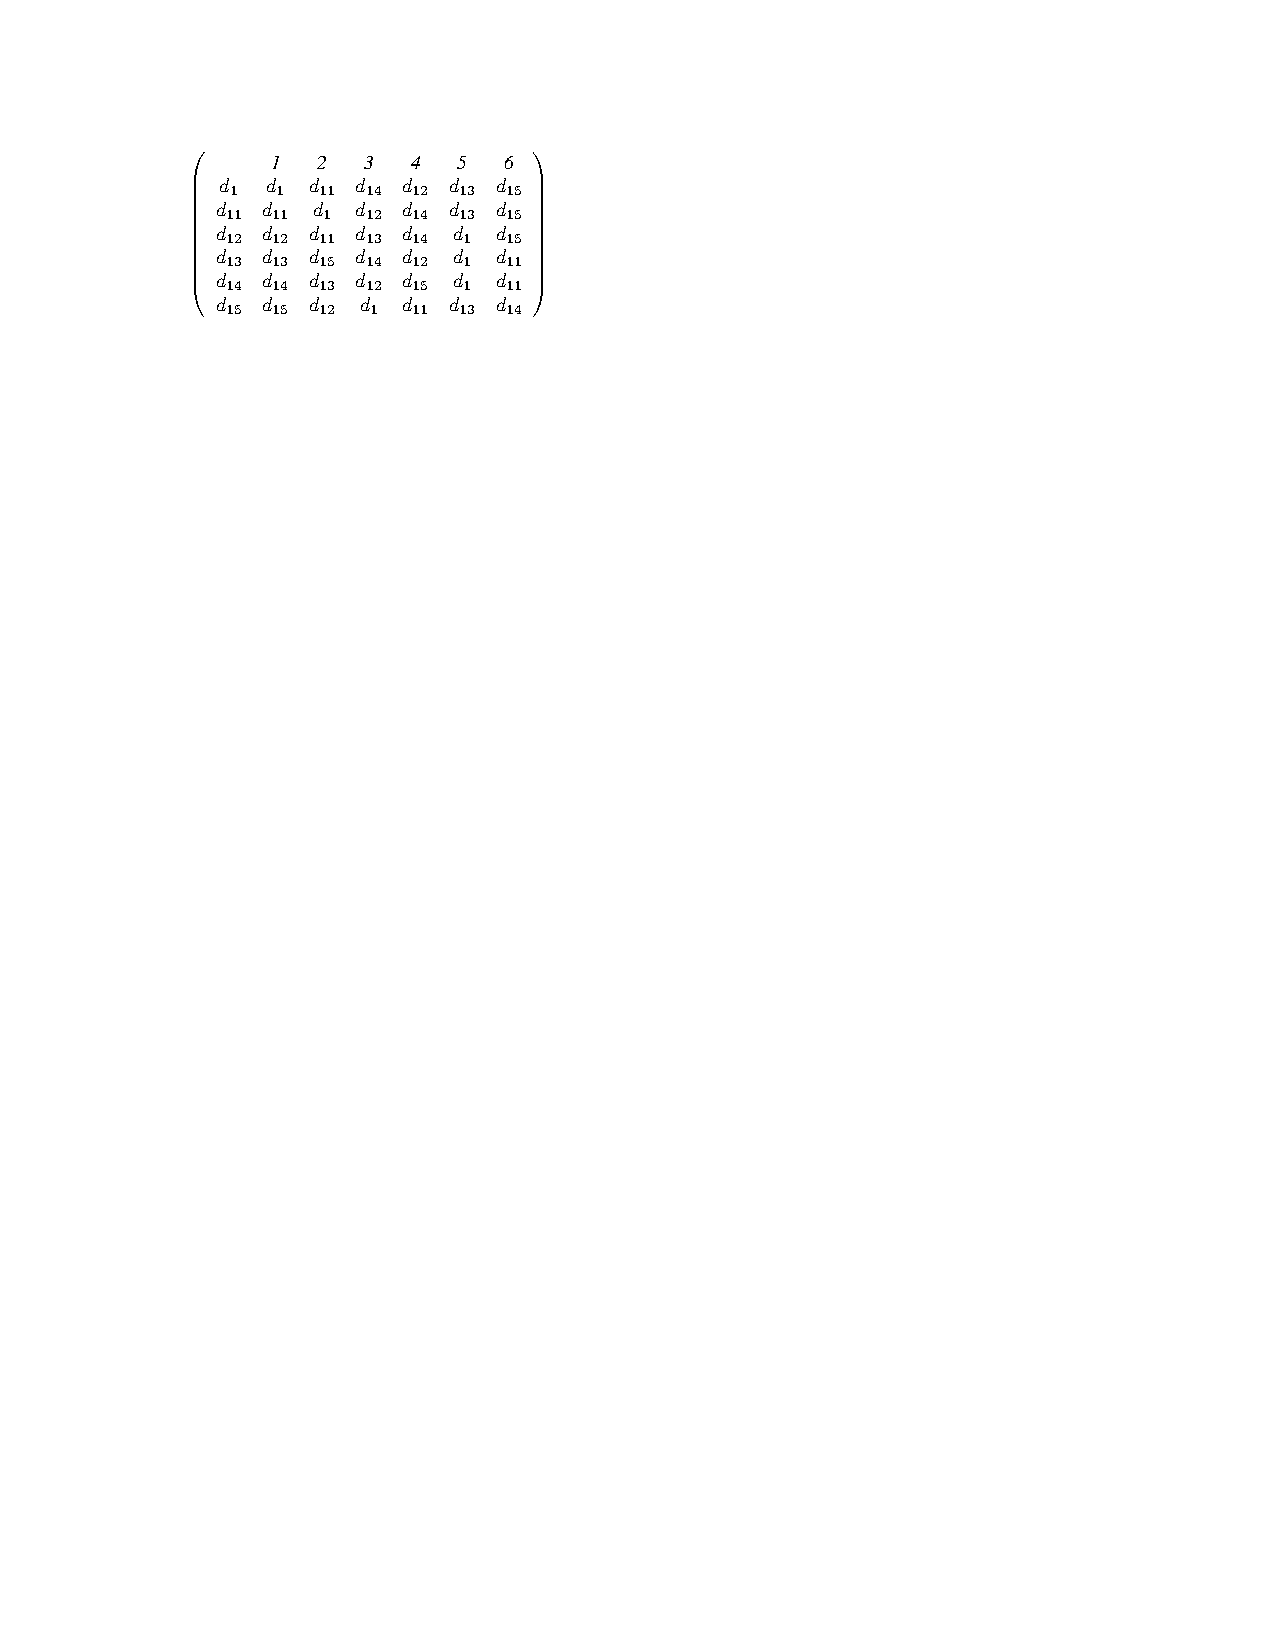
\includegraphics[width=\columnwidth]{figures/2-5/2-5-9.pdf}
  \end{figure}

\end{columns}

\begin{definition}[Distance Index Matrix]
\textrm{
\ssize{
an $N$-by-$N$ matrix, denoted as $M_{idx}$. Given a door identifier $d_i$, two integer $1 \leq j \leq k \leq N$, $M_{d2d}[d_i,M_{idx}[d_i, j]] \leq M_{d2d}[d_i,M_{idx}[d_i, k]]$.
}}
\end{definition}

\end{frame}

%------------------------------------------------

\begin{frame}
\frametitle{Indexing Indoor Moving Objects}

\begin{itemize}

\item store objects within the same partition together in an object bucket or several chained buckets.\\~\\

\item a linear table \conceptbf{Door-to-Partition Table} (DPT) is used to store the relationship between doors and partition object bucket. Each record in DPT is a 5-tuple $(d_i, vPtr_1, dist_1, vPtr_2, dist_2)$, where $d_i$ is a door identifier.\\~\\

\item if $D2P(d_i) = \{ (v_j, v_k) \}$, which means that door $d_i$ is directional from partition $v_j$ to $v_k$, then field $vPtr_1$ is a null pointer while $vPtr_2$ is a pointer that points to the object bucket of partition $v_k$, $dist_1$ is $\infty$, and $dist_2$ is $G_{dist}.f_{dv}(d_i, v_k)$.

\end{itemize}

\end{frame}

%------------------------------------------------

\begin{frame}
\frametitle{Intra-Partition Object Index and Search}

\begin{itemize}

\item a grid index is built for spatial objects in each indoor partition.\\~\\

\item all spatial objects in an indoor partition $v_i$ are organized using a corresponding bucket $B_i$, $B_i$ consists of multiple sub-buckets each of which corresponds to a grid cell.\\~\\

\item for $rangeSearch(B_i,q,r)$, search only those grid cells that overlap the circle centered at $q$ and with radius $r$, if a cell is fully inside the circle, all the objects in its sub-bucket are included directly.\\~\\

\item for $nnSearch(B_i, q, dist_{nn})$, search only those grid cells that overlap the circle centered at $q$ and with radius $dist_{nn}$.

\end{itemize}

\end{frame}


%------------------------------------------------

\begin{frame}
\frametitle{Indoor Distance-Aware Queries: \emph{Range Query}}

\begin{columns}[c]

  \column{0.5\textwidth}
  \begin{figure}[tb]
    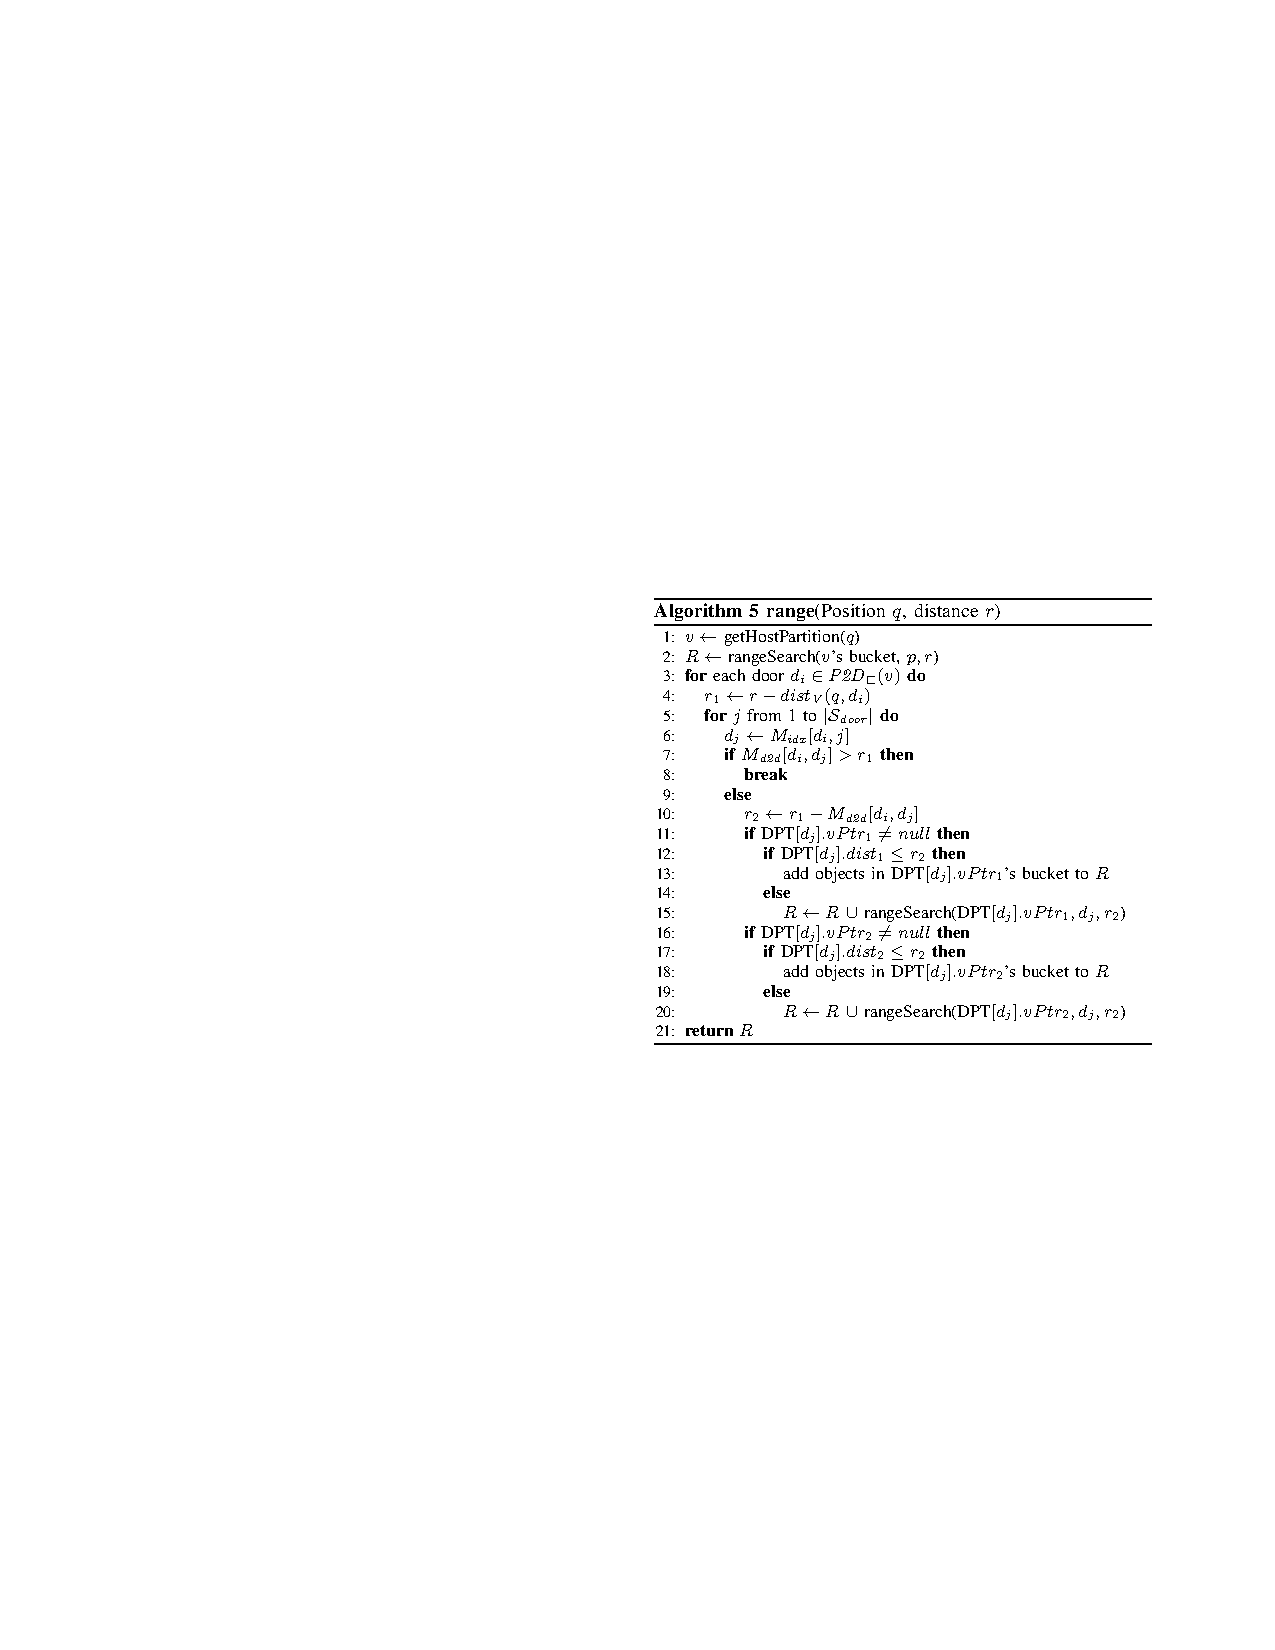
\includegraphics[width=\columnwidth]{figures/2-5/2-5-10.pdf}
  \end{figure}

  \column{0.5\textwidth}
  \ssize{
  \begin{enumerate}
    \item a range query $Q_r(q,r)$ returns those indoor objects that are within distance $r$ of $q$.
    \item lines 1--2: first gets the query position $q$'s host partition $v$ and searches for possibly qualifying objects within $v$ by calling $rangeSearch(v$\textrm{'s} $bucket, p, r)$.
    \item lines 4--8: exploiting the index in $M_{idx}[d_i, *]$, the search is conducted in non-descending order of $M_{idx}[d_i, d_j]$, where $d_j$ is a door covered by the distance $r$ from position $q$.
    \item lines 12--18: if a partition is entirely within the query range, all objects in corresponding bucket are added to the result.
  \end{enumerate}
  }

\end{columns}

\end{frame}

%------------------------------------------------

\begin{frame}
\frametitle{Indoor Distance-Aware Queries: \emph{Nearest Neighbor Query}}

\begin{columns}[c]

  \column{0.5\textwidth}
  \begin{figure}[tb]
    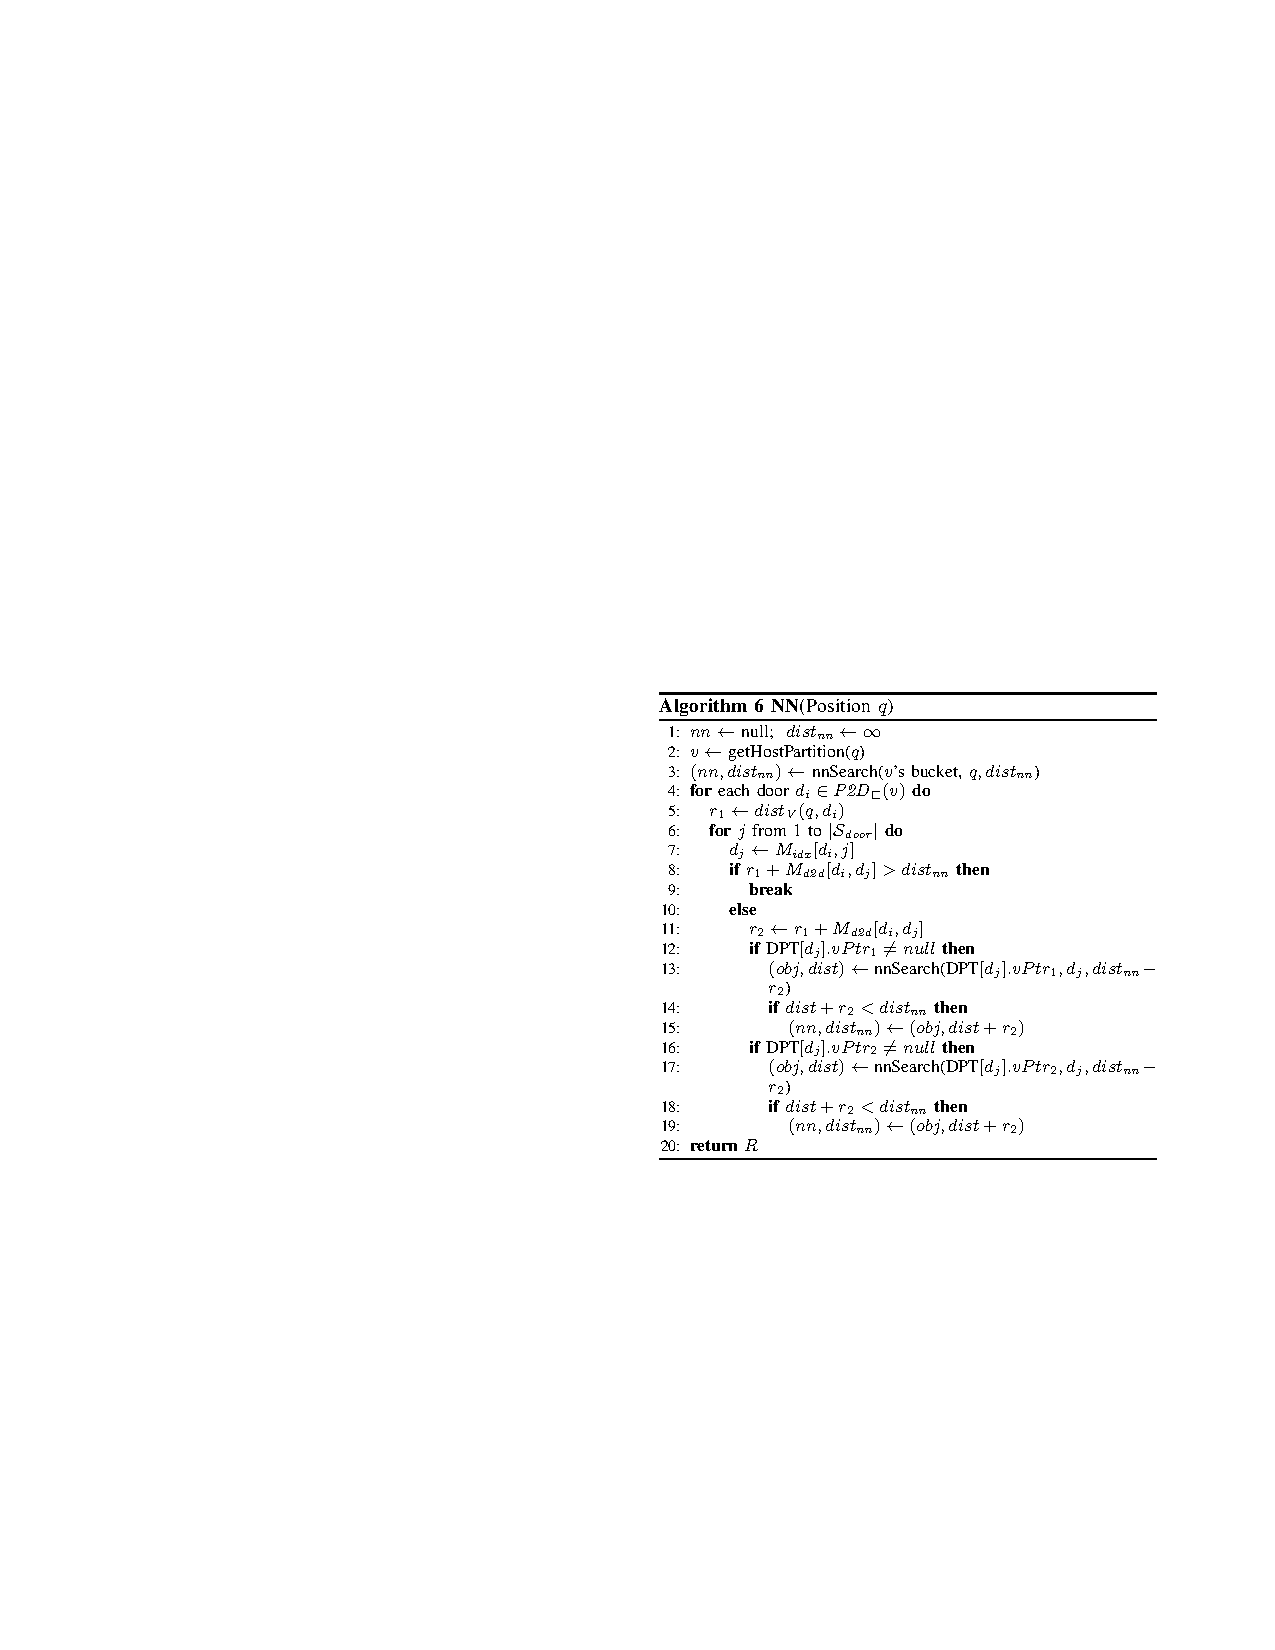
\includegraphics[width=\columnwidth]{figures/2-5/2-5-11.pdf}
  \end{figure}

  \column{0.5\textwidth}
  \ssize{
  \begin{enumerate}
    \item a nearest neighbor query $Q_{nn}(q,r)$ returns those indoor objects whose distance from $q$ is the samllest among all objects.
    \item line 2: $nnSearch(B_i, q, dist_{nn})$ searches an object bucket $B_i$ to find the nearest neighbor from $q$, $dist_{nn}$ is the current shortest distance for fast prunning.
    \item lines 4--19: for each door $d_i$ through which one can leave $v$, search is conducted in the similar way as for range query processing.
  \end{enumerate}
  }

\end{columns}

\end{frame}
